\chapter{Kravspecifikation}

\textbf{Versionshistorik}
\begin{longtabu} to \linewidth{@{}l l l X[j]@{}}
    Version &    Dato &    Ansvarlig &    Beskrivelse\\[-1ex]
    \midrule
    1.0		&	23-09-2015 &		Alle	&	Første udkast til Use Cases. I alt 4, hvor en af funktionaliteterne var, at man kunne optage en lydsekvens\\[-1ex]
    1.1		&	29-09-2015	&	Alle	&	Ændring af Use Cases efter møde med Peter. I alt 5, hvor funktionaliteterne kunne dækker over de opstillede krav til projektet. \\[-1ex]
    1.2		&	30-09-2015	&	Alle	&	Små ændring af formuleringerne samt byttet om på UC1 og UC2 og tilføjet en UC6. De ikke-funktionelle krav er blevet tilføjet. Klar til Review\\[-1ex]	
    2.0		&	08-10-2015	& Alle		&	Rettelser efter review møde\\[-1ex] 

\label{version_Systemark}
\end{longtabu}

\section{Indledning}
Kravspecifikationen vil gennem seks Use Cases beskrive blodtryksmålerens funktionelle krav. Systemets ikke-funktionelle krav er udarbejdet på baggrund af (F)URPS+. Dertil vil der være aktør-kontekst- og Use Casesdiagram samt beskrivelse af de forskellige aktører, der intergerer med systemet.  

\section{Systembeskrivelse}
 Systemet skal kunne vise et blodtryksignal kontinuert i en graf. Derudover skal systemet kunne kalibrere, nulpunktsjustere samt gemme data for målingen i en lokal database. Systemet er udvilket som en prototype, der er mulig at teste udfra de givne rammer. 

\section{Funktionelle krav}
De funktionelle krav vil nedenstående beskrives ud fra Aktør-kontekstdiagram, aktørbeskrivelse, Use Cases samt Use Case diagram. 

\subsection{Aktør-kontekstdiagram}
\begin{figure}[H]
	\centering
	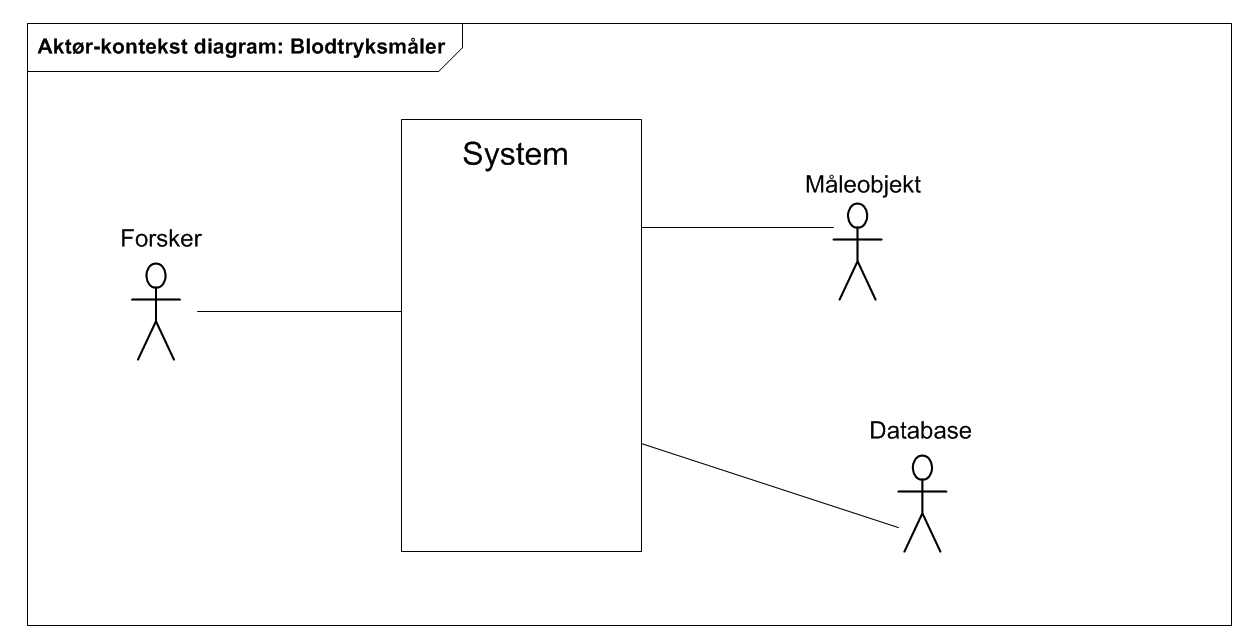
\includegraphics[width=1\textwidth]{Figurer/Snip20151027_47}
	\caption{Aktør-kontekstdiagram}
	\label{fig:aktoerbeskrivelse}
\end{figure}

Systemet består af en software- og en hardward-del. Softwaredelen er udarbejdet i Visual Studio C\#. Hardwaredelen består af flere komponenter sat sammen. Tryktransducer, Instrumentationforstærker, et aktivt 2. ordens lavpasfilter af typen Sallen-Key med unity gain og en DAQ. Det er selve systemet. \\
Primær aktøren i dette projekt er en Forsker. Sekundære aktører er Database og Måleobjekt. Måleobjekt er en package af Physionet og Analog Discovery, som er eksterne aktører.   

\subsection{Aktørbeskrivelse}

\begin{table}[H]
\begin{tabularx}{\textwidth}{l X}
     Aktørnavn & Forsker \\
     Type & Primær \\
     Beskrivelse  & Person med relevant baggrundsviden inden for blodtryksanalyse \\ 
     \midrule
     Aktørnavn & Måleobjekt  \\
     Type & Sekundær \\
     Beskrivelse  & Måleobjektet i det færdigudviklede produkt er et signal genereret enten in vitro eller in vivo. I prototypen er måleobjektet en kombination af Physionet og Analog Discovery. Måleobjektet repræsenterer data fra Physionet leveret til blodtryksmålingssystemet igennem Analog Discovery \\
     \midrule
     Aktørnavn & Database \\
     Type & Sekundær \\
     Beskrivelse  & Database bruges i blodtryksmålingssystemet til at gemme data \\ 
     \midrule
     Atørnavn & Physionet \\
     Type & Ekstern  \\
     Beskrivelse  & Physionet er en ekstern database, som indeholder blodtrykssignalet fra forskellige patienter \\
     \midrule
     Aktørnavn & Analog Discovery  \\
     Type & Ekstern \\
     Beskrivelse  & Analog Discovery omdanner data fra Physionet til at analogt signal \\                                                                                                                                                                          
     \bottomrule                                                                                                                   
    \end{tabularx}
    \caption {Aktørbeskrivelse}
    \label{tab:aktoerbeskrivelse}
	
\end{table}

\subsection{Use case-diagram}
\begin{figure}[H]
	\centering
	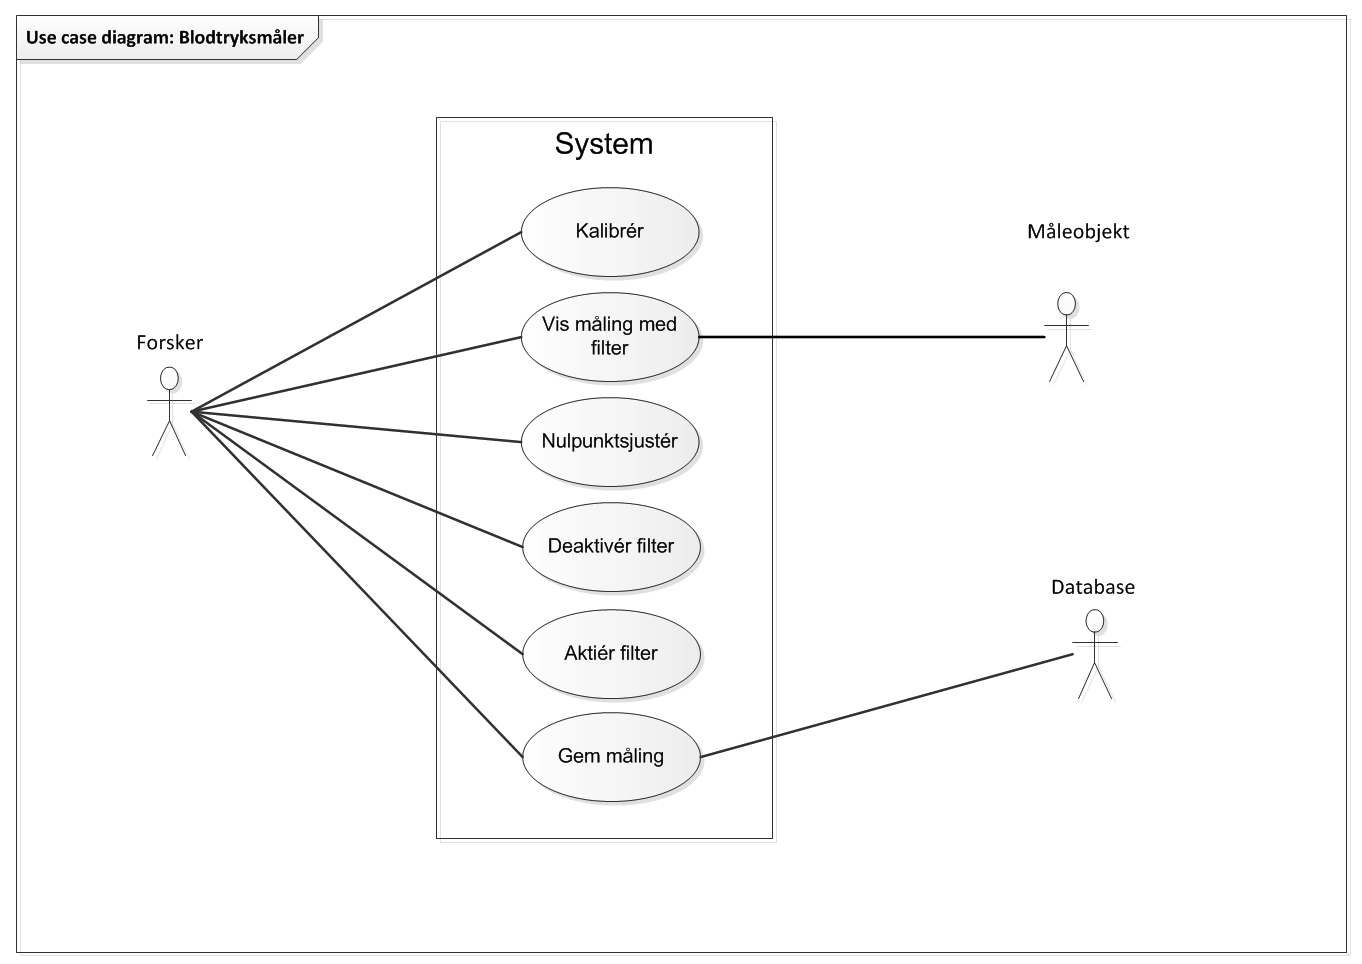
\includegraphics[width=1\textwidth]{Figurer/Snip20151027_49}
	\caption{Use case-diagram}
	\label{fig:Use case-diagram}
\end{figure}

Forskeren af systemet er den primære aktør i alle seks Use Cases. Det er Forskeren, der sætter alle Use Cases igang og styrer, hvad der skal ske og hvornår. Måleobjektet, som er den sekundære aktør, integrer i UC2, da det er her, blodtryksmålingen for Måleobjektet skal vises. For at få gemt data integrerer den sekundære aktør Database med UC6.  

\subsection{Use Cases}

\begin{longtabu} to \linewidth{@{}l r X[j]@{}} %UC1%
    {\large \textbf{Use Case 1}} && \\
    \toprule
    Navn &&    Kalibrér\\
    Use case ID &&    1\\
    Samtidige forløb &&    1\\
    Primær aktør &&    Forsker\\
    Sekundære aktør &&	 \\
    Mål &&    Forsker ønsker at kalibrere blodtrykssignal\\
    Initiering &&	Startes af Forsker\\
    Forudsætninger &&  System er aktivt og tilgængeligt\\
    Resultat &&		Blodtrykssignalet er kalibreret                         \\ \midrule
    Hovedforløb &    1. &	 Kalibrering-vinduet vises, hvor System spørger om der skal foretages en kalibrering\\[-1ex]  				
    			&    2. &    Forsker trykker på "Ja"\--knappen\newline
    						 [2.a \textit{Forsker trykker på "Nej"\--knappen}]\\
                &    3.	&	 System kalibrerer og Kalibrering-vinduet lukkes ned \newline\\ \midrule
                
    Undtagelser &    2.a &   Forsker ønsker ingen kalibrering. UC1 afsluttes og Kalibrering-vinduet lukkes  \\ \bottomrule
\caption{Fully dressed Use Case 1.}
\label{UC1}
\end{longtabu}


\begin{longtabu} to \linewidth{@{}l r X[j]@{}} %UC2%
    {\large \textbf{Use Case 2}} && \\
    \toprule
    Navn &&    Vis Måling med filter\\
    Use case ID &&    2\\
    Samtidige forløb &&    1\\
    Primær aktør &&    Forsker\\
    Sekundære aktør &&	 Måleobjekt\\
    Mål &&    Forsker ønsker at vise blodtrykssignal med digitalt filter\\
    Initiering &&	Startes af UC1\\
    Forudsætninger &&  System er aktivt og tilgængeligt. Digitalt filter er aktivt. Måleobjekt er tilsluttet system\\
    Resultat &&		Blodtrykssignalet udskrives                         \\ \midrule
    Hovedforløb &    1. &    Monitor-vinduet vises\\[-1ex]	
    			&    2. &    Blodtryksignal udskrives på en graf i 	  Monitor-vinduet\\[-1ex]
    			&	 3.	&	 Systole-, Diastole- og puls	værdier udskrives i Monitor-vinduet\newline\\ \midrule
                
    Undtagelser &    &   \\ \bottomrule
\caption{Fully dressed Use Case 2.}
\label{UC2}
\end{longtabu}


\begin{longtabu} to \linewidth{@{}l r X[j]@{}} %UC3%
    {\large \textbf{Use Case 3}} && \\
    \toprule
    Navn &&    Nulpunktsjustér\\
    Use case ID &&    3\\
    Samtidige forløb &&    1\\
    Primær aktør &&    Forsker\\
    Sekundære aktør && \\
    Mål &&    Forsker ønsker at nulpunktsjustere blodtrykssignal\\
    Initiering &&	Startes af Forsker\\
    Forudsætninger &&  System er aktivt og tilgængeligt. UC2 kører \\    Resultat &&		Blodtrykssignalet er nulpunktsjusteret\\ \midrule
    Hovedforløb &    1. &    Forsker trykker på "Nulpunktjustering"\--knappen\\[-1ex]   						 	
                &    2. &    System udfører nulpunktsjusteringen\\[-1ex]
                &	 3.	&	 Det fremgår i Monitor-vinduet, at nulpunktsjustering er foretaget\newline\\ \midrule
                
    Undtagelser &     &      \\ \bottomrule
\caption{Fully dressed Use Case 3.}
\label{UC3}
\end{longtabu}

\begin{longtabu} to \linewidth{@{}l r X[j]@{}} %UC4%
    {\large \textbf{Use Case 4}} && \\
    \toprule
    Navn &&    Deaktivér filter\\
    Use case ID &&    4\\
    Samtidige forløb &&   1\\
    Primær aktør &&    Forsker\\
    Sekundære aktør &&	 \\
    Mål &&    Forsker ønsker at deaktivere det digitale filter\\
    Initiering &&	Startes af Forsker\\
    Forudsætninger &&  System er aktivt og tilgængeligt. UC2 kører  \\
    Resultat &&		Ufiltreret blodtrykssignal vises i Monitor-vinduet                 \\ \midrule
    Hovedforløb &    1. &    Forsker deaktiverer filter ved at markere i \textit{" Deaktivér digitalt filtre"} \\[-1ex]   						 	
                &    2. &    System udskriver det ufiltreret blodtryksignal\newline\\ \midrule
                
    Undtagelser &     &      \\ \bottomrule
\caption{Fully dressed Use Case 4.}
\label{UC4}
\end{longtabu}


\begin{longtabu} to \linewidth{@{}l r X[j]@{}} %UC5%
    {\large \textbf{Use Case 5}} && \\
    \toprule
    Navn &&    Aktivér filter\\
    Use case ID &&    5\\
    Samtidige forløb &&   1\\
    Primær aktør &&    Forsker\\
    Sekundære aktør &&	 \\
    Mål &&    Forsker ønsker at aktivere det digitale filter\\
    Initiering &&	Startes af Forsker\\
    Forudsætninger &&  System er aktivt og tilgængeligt. Det digitale filter er deaktiveret  \\
    Resultat &&		Filtreret blodtrykssignal vises i Monitor-vindet                 \\ \midrule
    Hovedforløb &    1. &    Forsker aktiverer filter ved at markere i \textit{" Aktivér digitalt filtre"} \\[-1ex]   						 	
                &    2. &    System udskriver det filtreret blodtryksignal\newline\\ \midrule
                
    Undtagelser &     &      \\ \bottomrule
\caption{Fully dressed Use Case 5.}
\label{UC5}
\end{longtabu}
    
\begin{longtabu} to \linewidth{@{}l r X[j]@{}} %UC6%
    {\large \textbf{Use Case 6}} && \\
    \toprule
    Navn &&    Gem måling\\
    Use case ID &&    6\\
    Samtidige forløb &&   1.2...*\\
    Primær aktør &&    Forsker\\
    Sekundære aktør &&	Database\\
    Mål &&    Forsker ønsker at gemme data i Database\\
    Initiering &&	Startes af Forsker\\
    Forudsætninger &&  System er aktivt og tilgængeligt. UC2 kører  \\
    Resultat &&		Data er gemt i Database                 \\ \midrule
    Hovedforløb &    1. &    Forsker trykker på "Gem"\--knappen \newline
       						 [1.a \textit{Måleobjektets data er gemt fra forrige målinger}]\\	
                &    2. &    System åbner Gem-vinduet\\[-1ex]
                &    3.	&	 Forsker indtaster data for blodtryksmålingen \\[-1ex]
                &	 4. &    Forsker trykker på "OK"\--knappen  \\[-1ex]
                &	 5.	&	 System lukker Gem-vinduet og åbner Monitor-vinduet igen\\[-1ex]
                &	 6.	&	 System viser, at data er gemt i Monitor-vinduet\newline
                
                \\ \midrule
                
    Undtagelser &   1.a  &  UC6 forsættes ved punkt 6    \\ \bottomrule
\caption{Fully dressed Use Case 6.}
\label{UC6}
\end{longtabu}


\section{Ikke-funktionelle krav}
De ikke-funktionelle krav er specificeret ved brug af redskabet (F)URPS+, der står for hhv. Functionality, Usability, Reliability, Performance, Supportability og andre krav til fx brugssituationer og interface.  


\subsection{Functionality}
\begin{itemize}
	\item System skal kunne vise en kontinuerlig blodtryksignal i Monitor-vinduet.
	\item System skal kunne vise Systole-, Diastole- og Pulsværdier med op til tre cifre.
	\item System skal kunne vise et blodtrykssignal med og uden et digitalt filter.
	\item System skal kunne nulpunktsjustere blodtrykssignalet.
	\item System skal kunne gemme en blodtryksmåling i en database.
	\item System skal kunne kalibreres. 
\end{itemize}

\subsection{Usability}
\begin{itemize}
	\item Monitor-vinduet skal indeholde en ”Gem”\--knap.
	\item Monitor-vinduet skal indeholde en ”Nulpunktsjustér”\--knap.
	\item Monitor-vinduet skal indeholde et tidsstempel for seneste nulpunktsjustering.
	\item Monitor-vinduet skal indeholde to radiobuttons til aktivering og deaktivering af digitalt filter.
	\item Kalibrering-vinduet skal indeholde en ”Ja”\--knap og en ”Nej”\--knap.
	\item Kalibrering-vinduet skal indeholde et datostempel for seneste kalibrering.
	\item Gem-vinduet skal indeholde tekstbokse til data indtastning for målingen. 
	\item Gem-vinduet skal indeholde en ”OK”\--knap.
	\item Det skal være muligt at aflæse værdier på Monitor-vinduet fra 2 meters afstand med normalt syn.
\end{itemize}

\subsection{Reliability}
\begin{itemize}
	\item Systemet skal have en effektiv MTBF (Mean Time Between Failure) på 99 timer og en MTTR (Mean Time To Restore) på 20 minutter (1/3 time).
				\begin{align}
					Availability = \frac{MTBF}{MTBF+MTTR} = \frac{99}{99+1/3} = 0,997 = 99,7 \%
				\end{align}

\end{itemize}

\subsection{Performance}
\begin{itemize}
	\item Blodtrykssignalet skal vises maksimalt 5 sekunder efter UC1 er afsluttet.
	\item Systemet skal vise en graf for blodtryksmålingen, hvor y-aksen er mmHg og x-aksen er tid i sekunder.
	\item Systemet skal kunne måle blodtryksværdier fra 0 til 300 mmHg.
\end{itemize}

\subsection{Supportability}
\begin{itemize}
	\item Softwaren skal opbygges efter trelagsmodellen.
\end{itemize}

\subsection{Andre(+)}
\textbf{Brugssituationer}
\begin{itemize}
	\item Der skal være adgang til en computer med Windows 7 eller nyere – computeren skal have minimum 4 GB RAM.
	\item Der skal være adgang til en computer, hvor National Instruments er installeret.
\end{itemize}
\textbf{Interface}
\begin{itemize}
	\item Blodtryksdiagrammet skal fylde minimum 1/3 af Monitor-vinduet.
	\item Baggrunden i Monitor-vinduet skal være mørk.
	\item Blodtrykssignal og -værdier(systole og diastole) skal være røde, og puls skal være grøn.
	\item Systolisk og diastolisk blodtryk skal fremhæves øverst i højre hjørne ved større skriftstørrelse end andre værdier i Monitor-vinduet (fx værdier på akserne).
\end{itemize}













